\section{Model Selection}
\label{sec:model-selection}
	
	
	
	\subsection{Calibration}
	\label{ssec:calibration}

		\begin{figure*}
			\begin{subfigure}[b]{\textwidth}
				\centering
				% GNUPLOT: LaTeX picture with Postscript
\begingroup
  \makeatletter
  \providecommand\color[2][]{%
    \GenericError{(gnuplot) \space\space\space\@spaces}{%
      Package color not loaded in conjunction with
      terminal option `colourtext'%
    }{See the gnuplot documentation for explanation.%
    }{Either use 'blacktext' in gnuplot or load the package
      color.sty in LaTeX.}%
    \renewcommand\color[2][]{}%
  }%
  \providecommand\includegraphics[2][]{%
    \GenericError{(gnuplot) \space\space\space\@spaces}{%
      Package graphicx or graphics not loaded%
    }{See the gnuplot documentation for explanation.%
    }{The gnuplot epslatex terminal needs graphicx.sty or graphics.sty.}%
    \renewcommand\includegraphics[2][]{}%
  }%
  \providecommand\rotatebox[2]{#2}%
  \@ifundefined{ifGPcolor}{%
    \newif\ifGPcolor
    \GPcolorfalse
  }{}%
  \@ifundefined{ifGPblacktext}{%
    \newif\ifGPblacktext
    \GPblacktexttrue
  }{}%
  % define a \g@addto@macro without @ in the name:
  \let\gplgaddtomacro\g@addto@macro
  % define empty templates for all commands taking text:
  \gdef\gplbacktext{}%
  \gdef\gplfronttext{}%
  \makeatother
  \ifGPblacktext
    % no textcolor at all
    \def\colorrgb#1{}%
    \def\colorgray#1{}%
  \else
    % gray or color?
    \ifGPcolor
      \def\colorrgb#1{\color[rgb]{#1}}%
      \def\colorgray#1{\color[gray]{#1}}%
      \expandafter\def\csname LTw\endcsname{\color{white}}%
      \expandafter\def\csname LTb\endcsname{\color{black}}%
      \expandafter\def\csname LTa\endcsname{\color{black}}%
      \expandafter\def\csname LT0\endcsname{\color[rgb]{1,0,0}}%
      \expandafter\def\csname LT1\endcsname{\color[rgb]{0,1,0}}%
      \expandafter\def\csname LT2\endcsname{\color[rgb]{0,0,1}}%
      \expandafter\def\csname LT3\endcsname{\color[rgb]{1,0,1}}%
      \expandafter\def\csname LT4\endcsname{\color[rgb]{0,1,1}}%
      \expandafter\def\csname LT5\endcsname{\color[rgb]{1,1,0}}%
      \expandafter\def\csname LT6\endcsname{\color[rgb]{0,0,0}}%
      \expandafter\def\csname LT7\endcsname{\color[rgb]{1,0.3,0}}%
      \expandafter\def\csname LT8\endcsname{\color[rgb]{0.5,0.5,0.5}}%
    \else
      % gray
      \def\colorrgb#1{\color{black}}%
      \def\colorgray#1{\color[gray]{#1}}%
      \expandafter\def\csname LTw\endcsname{\color{white}}%
      \expandafter\def\csname LTb\endcsname{\color{black}}%
      \expandafter\def\csname LTa\endcsname{\color{black}}%
      \expandafter\def\csname LT0\endcsname{\color{black}}%
      \expandafter\def\csname LT1\endcsname{\color{black}}%
      \expandafter\def\csname LT2\endcsname{\color{black}}%
      \expandafter\def\csname LT3\endcsname{\color{black}}%
      \expandafter\def\csname LT4\endcsname{\color{black}}%
      \expandafter\def\csname LT5\endcsname{\color{black}}%
      \expandafter\def\csname LT6\endcsname{\color{black}}%
      \expandafter\def\csname LT7\endcsname{\color{black}}%
      \expandafter\def\csname LT8\endcsname{\color{black}}%
    \fi
  \fi
  \setlength{\unitlength}{0.0500bp}%
  \begin{picture}(7936.00,3400.00)%
    \gplgaddtomacro\gplbacktext{%
      \csname LTb\endcsname%
      \put(1078,704){\makebox(0,0)[r]{\strut{} 0.3}}%
      \csname LTb\endcsname%
      \put(1078,1190){\makebox(0,0)[r]{\strut{} 0.35}}%
      \csname LTb\endcsname%
      \put(1078,1676){\makebox(0,0)[r]{\strut{} 0.4}}%
      \csname LTb\endcsname%
      \put(1078,2163){\makebox(0,0)[r]{\strut{} 0.45}}%
      \csname LTb\endcsname%
      \put(1078,2649){\makebox(0,0)[r]{\strut{} 0.5}}%
      \csname LTb\endcsname%
      \put(1078,3135){\makebox(0,0)[r]{\strut{} 0.55}}%
      \csname LTb\endcsname%
      \put(1353,484){\makebox(0,0){\strut{} 1400}}%
      \csname LTb\endcsname%
      \put(2304,484){\makebox(0,0){\strut{} 1600}}%
      \csname LTb\endcsname%
      \put(3256,484){\makebox(0,0){\strut{} 1800}}%
      \csname LTb\endcsname%
      \put(4208,484){\makebox(0,0){\strut{} 2000}}%
      \csname LTb\endcsname%
      \put(5160,484){\makebox(0,0){\strut{} 2200}}%
      \csname LTb\endcsname%
      \put(6111,484){\makebox(0,0){\strut{} 2400}}%
      \csname LTb\endcsname%
      \put(7063,484){\makebox(0,0){\strut{} 2600}}%
      \put(176,1919){\rotatebox{-270}{\makebox(0,0){\strut{}$-\lg \varrho(\lambda)$}}}%
      \put(4374,154){\makebox(0,0){\strut{}$\lambda \ [\m{nm}]$}}%
    }%
    \gplgaddtomacro\gplfronttext{%
      \csname LTb\endcsname%
      \put(6587,2892){\makebox(0,0)[l]{\strut{}SOC}}%
    }%
    \gplbacktext
    \put(0,0){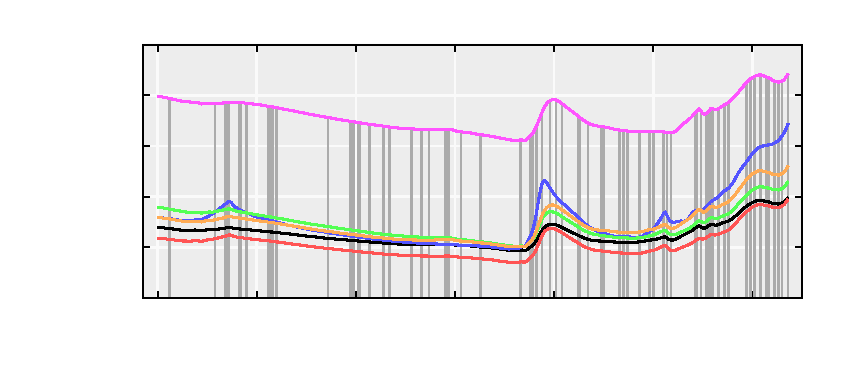
\includegraphics{gp/ms-sa-soc-spec-rnd}}%
    \gplfronttext
  \end{picture}%
\endgroup

				\caption{$p^{(\m{SOC})}$ with $\m{p}^{(\m{SOC})} = 72$}
				\label{sfig:calib-soc}
			\end{subfigure}
			
			\begin{subfigure}[b]{\textwidth}
				\centering
				% GNUPLOT: LaTeX picture with Postscript
\begingroup
  \makeatletter
  \providecommand\color[2][]{%
    \GenericError{(gnuplot) \space\space\space\@spaces}{%
      Package color not loaded in conjunction with
      terminal option `colourtext'%
    }{See the gnuplot documentation for explanation.%
    }{Either use 'blacktext' in gnuplot or load the package
      color.sty in LaTeX.}%
    \renewcommand\color[2][]{}%
  }%
  \providecommand\includegraphics[2][]{%
    \GenericError{(gnuplot) \space\space\space\@spaces}{%
      Package graphicx or graphics not loaded%
    }{See the gnuplot documentation for explanation.%
    }{The gnuplot epslatex terminal needs graphicx.sty or graphics.sty.}%
    \renewcommand\includegraphics[2][]{}%
  }%
  \providecommand\rotatebox[2]{#2}%
  \@ifundefined{ifGPcolor}{%
    \newif\ifGPcolor
    \GPcolorfalse
  }{}%
  \@ifundefined{ifGPblacktext}{%
    \newif\ifGPblacktext
    \GPblacktexttrue
  }{}%
  % define a \g@addto@macro without @ in the name:
  \let\gplgaddtomacro\g@addto@macro
  % define empty templates for all commands taking text:
  \gdef\gplbacktext{}%
  \gdef\gplfronttext{}%
  \makeatother
  \ifGPblacktext
    % no textcolor at all
    \def\colorrgb#1{}%
    \def\colorgray#1{}%
  \else
    % gray or color?
    \ifGPcolor
      \def\colorrgb#1{\color[rgb]{#1}}%
      \def\colorgray#1{\color[gray]{#1}}%
      \expandafter\def\csname LTw\endcsname{\color{white}}%
      \expandafter\def\csname LTb\endcsname{\color{black}}%
      \expandafter\def\csname LTa\endcsname{\color{black}}%
      \expandafter\def\csname LT0\endcsname{\color[rgb]{1,0,0}}%
      \expandafter\def\csname LT1\endcsname{\color[rgb]{0,1,0}}%
      \expandafter\def\csname LT2\endcsname{\color[rgb]{0,0,1}}%
      \expandafter\def\csname LT3\endcsname{\color[rgb]{1,0,1}}%
      \expandafter\def\csname LT4\endcsname{\color[rgb]{0,1,1}}%
      \expandafter\def\csname LT5\endcsname{\color[rgb]{1,1,0}}%
      \expandafter\def\csname LT6\endcsname{\color[rgb]{0,0,0}}%
      \expandafter\def\csname LT7\endcsname{\color[rgb]{1,0.3,0}}%
      \expandafter\def\csname LT8\endcsname{\color[rgb]{0.5,0.5,0.5}}%
    \else
      % gray
      \def\colorrgb#1{\color{black}}%
      \def\colorgray#1{\color[gray]{#1}}%
      \expandafter\def\csname LTw\endcsname{\color{white}}%
      \expandafter\def\csname LTb\endcsname{\color{black}}%
      \expandafter\def\csname LTa\endcsname{\color{black}}%
      \expandafter\def\csname LT0\endcsname{\color{black}}%
      \expandafter\def\csname LT1\endcsname{\color{black}}%
      \expandafter\def\csname LT2\endcsname{\color{black}}%
      \expandafter\def\csname LT3\endcsname{\color{black}}%
      \expandafter\def\csname LT4\endcsname{\color{black}}%
      \expandafter\def\csname LT5\endcsname{\color{black}}%
      \expandafter\def\csname LT6\endcsname{\color{black}}%
      \expandafter\def\csname LT7\endcsname{\color{black}}%
      \expandafter\def\csname LT8\endcsname{\color{black}}%
    \fi
  \fi
  \setlength{\unitlength}{0.0500bp}%
  \begin{picture}(7936.00,3400.00)%
    \gplgaddtomacro\gplbacktext{%
      \csname LTb\endcsname%
      \put(1078,704){\makebox(0,0)[r]{\strut{} 0.3}}%
      \csname LTb\endcsname%
      \put(1078,1190){\makebox(0,0)[r]{\strut{} 0.35}}%
      \csname LTb\endcsname%
      \put(1078,1676){\makebox(0,0)[r]{\strut{} 0.4}}%
      \csname LTb\endcsname%
      \put(1078,2163){\makebox(0,0)[r]{\strut{} 0.45}}%
      \csname LTb\endcsname%
      \put(1078,2649){\makebox(0,0)[r]{\strut{} 0.5}}%
      \csname LTb\endcsname%
      \put(1078,3135){\makebox(0,0)[r]{\strut{} 0.55}}%
      \csname LTb\endcsname%
      \put(1353,484){\makebox(0,0){\strut{} 1400}}%
      \csname LTb\endcsname%
      \put(2304,484){\makebox(0,0){\strut{} 1600}}%
      \csname LTb\endcsname%
      \put(3256,484){\makebox(0,0){\strut{} 1800}}%
      \csname LTb\endcsname%
      \put(4208,484){\makebox(0,0){\strut{} 2000}}%
      \csname LTb\endcsname%
      \put(5160,484){\makebox(0,0){\strut{} 2200}}%
      \csname LTb\endcsname%
      \put(6111,484){\makebox(0,0){\strut{} 2400}}%
      \csname LTb\endcsname%
      \put(7063,484){\makebox(0,0){\strut{} 2600}}%
      \put(176,1919){\rotatebox{-270}{\makebox(0,0){\strut{}$-\lg \varrho(\lambda)$}}}%
      \put(4374,154){\makebox(0,0){\strut{}$\lambda \ [\m{nm}]$}}%
    }%
    \gplgaddtomacro\gplfronttext{%
      \csname LTb\endcsname%
      \put(6587,2892){\makebox(0,0)[r]{\strut{}$P^\m{(N)}$}}%
    }%
    \gplbacktext
    \put(0,0){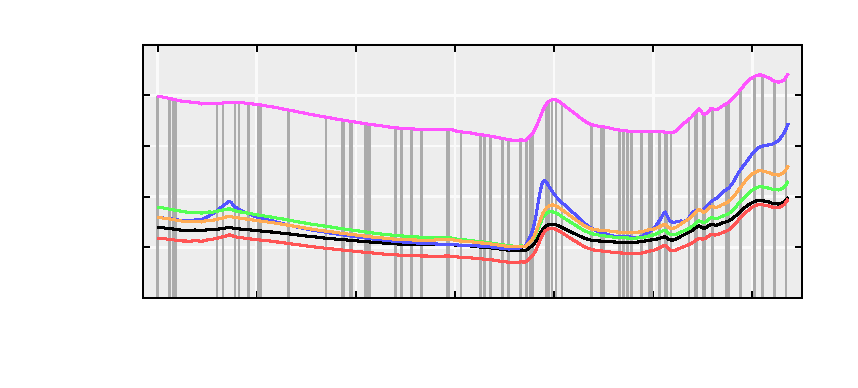
\includegraphics{gp/ms-sa-n-spec-rnd}}%
    \gplfronttext
  \end{picture}%
\endgroup

				\caption{$p^{(\m{N})}$ with $\m{p}^{(\m{N})} = 69$}
				\label{sfig:calib-n}
			\end{subfigure}

			\begin{subfigure}[b]{\textwidth}
				\centering
				% GNUPLOT: LaTeX picture with Postscript
\begingroup
  \makeatletter
  \providecommand\color[2][]{%
    \GenericError{(gnuplot) \space\space\space\@spaces}{%
      Package color not loaded in conjunction with
      terminal option `colourtext'%
    }{See the gnuplot documentation for explanation.%
    }{Either use 'blacktext' in gnuplot or load the package
      color.sty in LaTeX.}%
    \renewcommand\color[2][]{}%
  }%
  \providecommand\includegraphics[2][]{%
    \GenericError{(gnuplot) \space\space\space\@spaces}{%
      Package graphicx or graphics not loaded%
    }{See the gnuplot documentation for explanation.%
    }{The gnuplot epslatex terminal needs graphicx.sty or graphics.sty.}%
    \renewcommand\includegraphics[2][]{}%
  }%
  \providecommand\rotatebox[2]{#2}%
  \@ifundefined{ifGPcolor}{%
    \newif\ifGPcolor
    \GPcolorfalse
  }{}%
  \@ifundefined{ifGPblacktext}{%
    \newif\ifGPblacktext
    \GPblacktexttrue
  }{}%
  % define a \g@addto@macro without @ in the name:
  \let\gplgaddtomacro\g@addto@macro
  % define empty templates for all commands taking text:
  \gdef\gplbacktext{}%
  \gdef\gplfronttext{}%
  \makeatother
  \ifGPblacktext
    % no textcolor at all
    \def\colorrgb#1{}%
    \def\colorgray#1{}%
  \else
    % gray or color?
    \ifGPcolor
      \def\colorrgb#1{\color[rgb]{#1}}%
      \def\colorgray#1{\color[gray]{#1}}%
      \expandafter\def\csname LTw\endcsname{\color{white}}%
      \expandafter\def\csname LTb\endcsname{\color{black}}%
      \expandafter\def\csname LTa\endcsname{\color{black}}%
      \expandafter\def\csname LT0\endcsname{\color[rgb]{1,0,0}}%
      \expandafter\def\csname LT1\endcsname{\color[rgb]{0,1,0}}%
      \expandafter\def\csname LT2\endcsname{\color[rgb]{0,0,1}}%
      \expandafter\def\csname LT3\endcsname{\color[rgb]{1,0,1}}%
      \expandafter\def\csname LT4\endcsname{\color[rgb]{0,1,1}}%
      \expandafter\def\csname LT5\endcsname{\color[rgb]{1,1,0}}%
      \expandafter\def\csname LT6\endcsname{\color[rgb]{0,0,0}}%
      \expandafter\def\csname LT7\endcsname{\color[rgb]{1,0.3,0}}%
      \expandafter\def\csname LT8\endcsname{\color[rgb]{0.5,0.5,0.5}}%
    \else
      % gray
      \def\colorrgb#1{\color{black}}%
      \def\colorgray#1{\color[gray]{#1}}%
      \expandafter\def\csname LTw\endcsname{\color{white}}%
      \expandafter\def\csname LTb\endcsname{\color{black}}%
      \expandafter\def\csname LTa\endcsname{\color{black}}%
      \expandafter\def\csname LT0\endcsname{\color{black}}%
      \expandafter\def\csname LT1\endcsname{\color{black}}%
      \expandafter\def\csname LT2\endcsname{\color{black}}%
      \expandafter\def\csname LT3\endcsname{\color{black}}%
      \expandafter\def\csname LT4\endcsname{\color{black}}%
      \expandafter\def\csname LT5\endcsname{\color{black}}%
      \expandafter\def\csname LT6\endcsname{\color{black}}%
      \expandafter\def\csname LT7\endcsname{\color{black}}%
      \expandafter\def\csname LT8\endcsname{\color{black}}%
    \fi
  \fi
  \setlength{\unitlength}{0.0500bp}%
  \begin{picture}(7936.00,3400.00)%
    \gplgaddtomacro\gplbacktext{%
      \csname LTb\endcsname%
      \put(1078,704){\makebox(0,0)[r]{\strut{} 0.3}}%
      \csname LTb\endcsname%
      \put(1078,1190){\makebox(0,0)[r]{\strut{} 0.35}}%
      \csname LTb\endcsname%
      \put(1078,1676){\makebox(0,0)[r]{\strut{} 0.4}}%
      \csname LTb\endcsname%
      \put(1078,2163){\makebox(0,0)[r]{\strut{} 0.45}}%
      \csname LTb\endcsname%
      \put(1078,2649){\makebox(0,0)[r]{\strut{} 0.5}}%
      \csname LTb\endcsname%
      \put(1078,3135){\makebox(0,0)[r]{\strut{} 0.55}}%
      \csname LTb\endcsname%
      \put(1353,484){\makebox(0,0){\strut{} 1400}}%
      \csname LTb\endcsname%
      \put(2304,484){\makebox(0,0){\strut{} 1600}}%
      \csname LTb\endcsname%
      \put(3256,484){\makebox(0,0){\strut{} 1800}}%
      \csname LTb\endcsname%
      \put(4208,484){\makebox(0,0){\strut{} 2000}}%
      \csname LTb\endcsname%
      \put(5160,484){\makebox(0,0){\strut{} 2200}}%
      \csname LTb\endcsname%
      \put(6111,484){\makebox(0,0){\strut{} 2400}}%
      \csname LTb\endcsname%
      \put(7063,484){\makebox(0,0){\strut{} 2600}}%
      \put(176,1919){\rotatebox{-270}{\makebox(0,0){\strut{}$-\lg \varrho(\lambda)$}}}%
      \put(4374,154){\makebox(0,0){\strut{}$\lambda \ [\m{nm}]$}}%
    }%
    \gplgaddtomacro\gplfronttext{%
      \csname LTb\endcsname%
      \put(6587,2892){\makebox(0,0)[l]{\strut{}pH}}%
    }%
    \gplbacktext
    \put(0,0){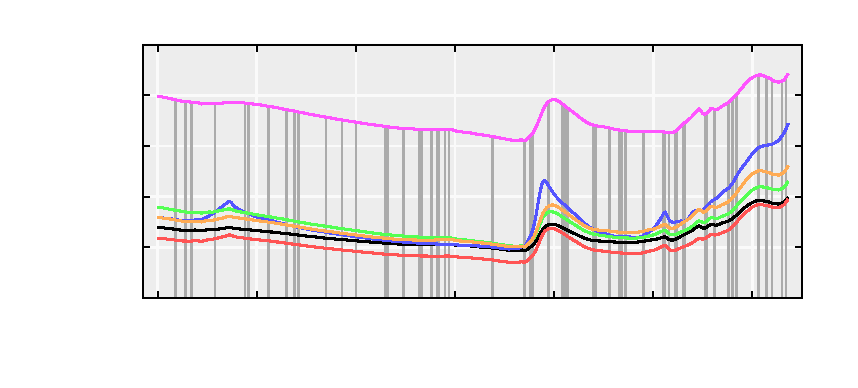
\includegraphics{gp/ms-sa-ph-spec-rnd}}%
    \gplfronttext
  \end{picture}%
\endgroup

				\caption{$\m{pH}$ with $\m{p}^{(\m{pH})} = 58$} % why again do we use a different notation in captions and on plots?
				\label{sfig:calib-ph}
			\end{subfigure}
			\caption{Displaying the spectra from figure \ref{fig:soil-spec-rnd} with wavelength included in the selected models for each response highlighted by vertical grey lines}
		\end{figure*}
				
		\begin{figure*}
			\center
			% \subcaphangtrue
			\begin{subfigure}[t]{0.33\textwidth}
				\centerline{
					% GNUPLOT: LaTeX picture with Postscript
\begingroup
  \makeatletter
  \providecommand\color[2][]{%
    \GenericError{(gnuplot) \space\space\space\@spaces}{%
      Package color not loaded in conjunction with
      terminal option `colourtext'%
    }{See the gnuplot documentation for explanation.%
    }{Either use 'blacktext' in gnuplot or load the package
      color.sty in LaTeX.}%
    \renewcommand\color[2][]{}%
  }%
  \providecommand\includegraphics[2][]{%
    \GenericError{(gnuplot) \space\space\space\@spaces}{%
      Package graphicx or graphics not loaded%
    }{See the gnuplot documentation for explanation.%
    }{The gnuplot epslatex terminal needs graphicx.sty or graphics.sty.}%
    \renewcommand\includegraphics[2][]{}%
  }%
  \providecommand\rotatebox[2]{#2}%
  \@ifundefined{ifGPcolor}{%
    \newif\ifGPcolor
    \GPcolorfalse
  }{}%
  \@ifundefined{ifGPblacktext}{%
    \newif\ifGPblacktext
    \GPblacktexttrue
  }{}%
  % define a \g@addto@macro without @ in the name:
  \let\gplgaddtomacro\g@addto@macro
  % define empty templates for all commands taking text:
  \gdef\gplbacktext{}%
  \gdef\gplfronttext{}%
  \makeatother
  \ifGPblacktext
    % no textcolor at all
    \def\colorrgb#1{}%
    \def\colorgray#1{}%
  \else
    % gray or color?
    \ifGPcolor
      \def\colorrgb#1{\color[rgb]{#1}}%
      \def\colorgray#1{\color[gray]{#1}}%
      \expandafter\def\csname LTw\endcsname{\color{white}}%
      \expandafter\def\csname LTb\endcsname{\color{black}}%
      \expandafter\def\csname LTa\endcsname{\color{black}}%
      \expandafter\def\csname LT0\endcsname{\color[rgb]{1,0,0}}%
      \expandafter\def\csname LT1\endcsname{\color[rgb]{0,1,0}}%
      \expandafter\def\csname LT2\endcsname{\color[rgb]{0,0,1}}%
      \expandafter\def\csname LT3\endcsname{\color[rgb]{1,0,1}}%
      \expandafter\def\csname LT4\endcsname{\color[rgb]{0,1,1}}%
      \expandafter\def\csname LT5\endcsname{\color[rgb]{1,1,0}}%
      \expandafter\def\csname LT6\endcsname{\color[rgb]{0,0,0}}%
      \expandafter\def\csname LT7\endcsname{\color[rgb]{1,0.3,0}}%
      \expandafter\def\csname LT8\endcsname{\color[rgb]{0.5,0.5,0.5}}%
    \else
      % gray
      \def\colorrgb#1{\color{black}}%
      \def\colorgray#1{\color[gray]{#1}}%
      \expandafter\def\csname LTw\endcsname{\color{white}}%
      \expandafter\def\csname LTb\endcsname{\color{black}}%
      \expandafter\def\csname LTa\endcsname{\color{black}}%
      \expandafter\def\csname LT0\endcsname{\color{black}}%
      \expandafter\def\csname LT1\endcsname{\color{black}}%
      \expandafter\def\csname LT2\endcsname{\color{black}}%
      \expandafter\def\csname LT3\endcsname{\color{black}}%
      \expandafter\def\csname LT4\endcsname{\color{black}}%
      \expandafter\def\csname LT5\endcsname{\color{black}}%
      \expandafter\def\csname LT6\endcsname{\color{black}}%
      \expandafter\def\csname LT7\endcsname{\color{black}}%
      \expandafter\def\csname LT8\endcsname{\color{black}}%
    \fi
  \fi
  \setlength{\unitlength}{0.0500bp}%
  \begin{picture}(3118.00,2834.00)%
    \gplgaddtomacro\gplbacktext{%
      \csname LTb\endcsname%
      \put(594,688){\makebox(0,0)[r]{\strut{} 0}}%
      \csname LTb\endcsname%
      \put(594,1051){\makebox(0,0)[r]{\strut{} 2}}%
      \csname LTb\endcsname%
      \put(594,1414){\makebox(0,0)[r]{\strut{} 4}}%
      \csname LTb\endcsname%
      \put(594,1777){\makebox(0,0)[r]{\strut{} 6}}%
      \csname LTb\endcsname%
      \put(594,2139){\makebox(0,0)[r]{\strut{} 8}}%
      \csname LTb\endcsname%
      \put(594,2502){\makebox(0,0)[r]{\strut{} 10}}%
      \csname LTb\endcsname%
      \put(907,287){\makebox(0,0){\strut{} 0}}%
      \csname LTb\endcsname%
      \put(1270,287){\makebox(0,0){\strut{} 2}}%
      \csname LTb\endcsname%
      \put(1633,287){\makebox(0,0){\strut{} 4}}%
      \csname LTb\endcsname%
      \put(1996,287){\makebox(0,0){\strut{} 6}}%
      \csname LTb\endcsname%
      \put(2358,287){\makebox(0,0){\strut{} 8}}%
      \csname LTb\endcsname%
      \put(2721,287){\makebox(0,0){\strut{} 10}}%
    }%
    \gplgaddtomacro\gplfronttext{%
      \csname LTb\endcsname%
      \put(1089,2139){\makebox(0,0)[l]{\strut{}SOC}}%
    }%
    \gplbacktext
    \put(0,0){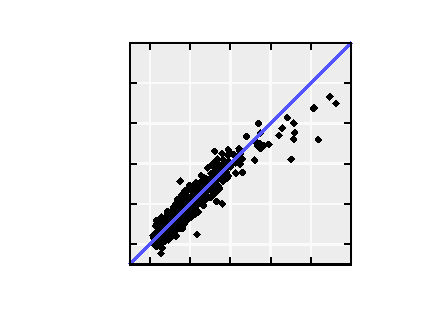
\includegraphics{gp/ms-sa-soc-corr}}%
    \gplfronttext
  \end{picture}%
\endgroup

				}
				\caption{\parbox[t]{0.45\textwidth}{
					$\hat{p}^{(\m{SOC})} \sim p^{(\m{SOC})}$ \smallskip \\
					$(R^2)^{(\m{SOC})} = 0.871$
					}}
			\end{subfigure}
			\begin{subfigure}[t]{0.33\textwidth}
				\centerline{
					% GNUPLOT: LaTeX picture with Postscript
\begingroup
  \makeatletter
  \providecommand\color[2][]{%
    \GenericError{(gnuplot) \space\space\space\@spaces}{%
      Package color not loaded in conjunction with
      terminal option `colourtext'%
    }{See the gnuplot documentation for explanation.%
    }{Either use 'blacktext' in gnuplot or load the package
      color.sty in LaTeX.}%
    \renewcommand\color[2][]{}%
  }%
  \providecommand\includegraphics[2][]{%
    \GenericError{(gnuplot) \space\space\space\@spaces}{%
      Package graphicx or graphics not loaded%
    }{See the gnuplot documentation for explanation.%
    }{The gnuplot epslatex terminal needs graphicx.sty or graphics.sty.}%
    \renewcommand\includegraphics[2][]{}%
  }%
  \providecommand\rotatebox[2]{#2}%
  \@ifundefined{ifGPcolor}{%
    \newif\ifGPcolor
    \GPcolorfalse
  }{}%
  \@ifundefined{ifGPblacktext}{%
    \newif\ifGPblacktext
    \GPblacktexttrue
  }{}%
  % define a \g@addto@macro without @ in the name:
  \let\gplgaddtomacro\g@addto@macro
  % define empty templates for all commands taking text:
  \gdef\gplbacktext{}%
  \gdef\gplfronttext{}%
  \makeatother
  \ifGPblacktext
    % no textcolor at all
    \def\colorrgb#1{}%
    \def\colorgray#1{}%
  \else
    % gray or color?
    \ifGPcolor
      \def\colorrgb#1{\color[rgb]{#1}}%
      \def\colorgray#1{\color[gray]{#1}}%
      \expandafter\def\csname LTw\endcsname{\color{white}}%
      \expandafter\def\csname LTb\endcsname{\color{black}}%
      \expandafter\def\csname LTa\endcsname{\color{black}}%
      \expandafter\def\csname LT0\endcsname{\color[rgb]{1,0,0}}%
      \expandafter\def\csname LT1\endcsname{\color[rgb]{0,1,0}}%
      \expandafter\def\csname LT2\endcsname{\color[rgb]{0,0,1}}%
      \expandafter\def\csname LT3\endcsname{\color[rgb]{1,0,1}}%
      \expandafter\def\csname LT4\endcsname{\color[rgb]{0,1,1}}%
      \expandafter\def\csname LT5\endcsname{\color[rgb]{1,1,0}}%
      \expandafter\def\csname LT6\endcsname{\color[rgb]{0,0,0}}%
      \expandafter\def\csname LT7\endcsname{\color[rgb]{1,0.3,0}}%
      \expandafter\def\csname LT8\endcsname{\color[rgb]{0.5,0.5,0.5}}%
    \else
      % gray
      \def\colorrgb#1{\color{black}}%
      \def\colorgray#1{\color[gray]{#1}}%
      \expandafter\def\csname LTw\endcsname{\color{white}}%
      \expandafter\def\csname LTb\endcsname{\color{black}}%
      \expandafter\def\csname LTa\endcsname{\color{black}}%
      \expandafter\def\csname LT0\endcsname{\color{black}}%
      \expandafter\def\csname LT1\endcsname{\color{black}}%
      \expandafter\def\csname LT2\endcsname{\color{black}}%
      \expandafter\def\csname LT3\endcsname{\color{black}}%
      \expandafter\def\csname LT4\endcsname{\color{black}}%
      \expandafter\def\csname LT5\endcsname{\color{black}}%
      \expandafter\def\csname LT6\endcsname{\color{black}}%
      \expandafter\def\csname LT7\endcsname{\color{black}}%
      \expandafter\def\csname LT8\endcsname{\color{black}}%
    \fi
  \fi
  \setlength{\unitlength}{0.0500bp}%
  \begin{picture}(3968.00,2834.00)%
    \gplgaddtomacro\gplbacktext{%
      \csname LTb\endcsname%
      \put(1018,677){\makebox(0,0)[r]{\strut{} 0}}%
      \csname LTb\endcsname%
      \put(1018,1150){\makebox(0,0)[r]{\strut{} 0.2}}%
      \csname LTb\endcsname%
      \put(1018,1623){\makebox(0,0)[r]{\strut{} 0.4}}%
      \csname LTb\endcsname%
      \put(1018,2096){\makebox(0,0)[r]{\strut{} 0.6}}%
      \csname LTb\endcsname%
      \put(1018,2569){\makebox(0,0)[r]{\strut{} 0.8}}%
      \csname LTb\endcsname%
      \put(1387,220){\makebox(0,0){\strut{} 0}}%
      \csname LTb\endcsname%
      \put(1860,220){\makebox(0,0){\strut{} 0.2}}%
      \csname LTb\endcsname%
      \put(2333,220){\makebox(0,0){\strut{} 0.4}}%
      \csname LTb\endcsname%
      \put(2806,220){\makebox(0,0){\strut{} 0.6}}%
      \csname LTb\endcsname%
      \put(3279,220){\makebox(0,0){\strut{} 0.8}}%
    }%
    \gplgaddtomacro\gplfronttext{%
      \csname LTb\endcsname%
      \put(1469,2250){\makebox(0,0)[l]{\strut{}$P^\m{(N)}$}}%
    }%
    \gplbacktext
    \put(0,0){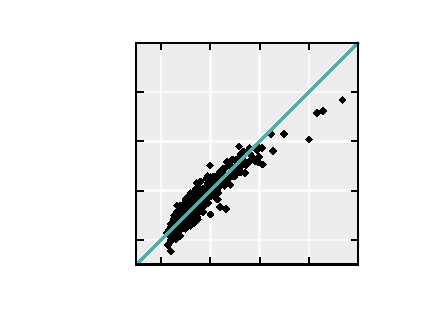
\includegraphics{gp/ms-sa-n-corr}}%
    \gplfronttext
  \end{picture}%
\endgroup

				}
				\caption{\parbox[t]{0.4\textwidth}{
					$\hat{p}^{(\m{N})} \sim p^{(\m{N})}$ \smallskip \\
					$(R^2)^{(\m{N})} = 0.861$
					}}
			\end{subfigure}
			\begin{subfigure}[t]{0.33\textwidth}
				\centerline{
					% GNUPLOT: LaTeX picture with Postscript
\begingroup
  \makeatletter
  \providecommand\color[2][]{%
    \GenericError{(gnuplot) \space\space\space\@spaces}{%
      Package color not loaded in conjunction with
      terminal option `colourtext'%
    }{See the gnuplot documentation for explanation.%
    }{Either use 'blacktext' in gnuplot or load the package
      color.sty in LaTeX.}%
    \renewcommand\color[2][]{}%
  }%
  \providecommand\includegraphics[2][]{%
    \GenericError{(gnuplot) \space\space\space\@spaces}{%
      Package graphicx or graphics not loaded%
    }{See the gnuplot documentation for explanation.%
    }{The gnuplot epslatex terminal needs graphicx.sty or graphics.sty.}%
    \renewcommand\includegraphics[2][]{}%
  }%
  \providecommand\rotatebox[2]{#2}%
  \@ifundefined{ifGPcolor}{%
    \newif\ifGPcolor
    \GPcolorfalse
  }{}%
  \@ifundefined{ifGPblacktext}{%
    \newif\ifGPblacktext
    \GPblacktexttrue
  }{}%
  % define a \g@addto@macro without @ in the name:
  \let\gplgaddtomacro\g@addto@macro
  % define empty templates for all commands taking text:
  \gdef\gplbacktext{}%
  \gdef\gplfronttext{}%
  \makeatother
  \ifGPblacktext
    % no textcolor at all
    \def\colorrgb#1{}%
    \def\colorgray#1{}%
  \else
    % gray or color?
    \ifGPcolor
      \def\colorrgb#1{\color[rgb]{#1}}%
      \def\colorgray#1{\color[gray]{#1}}%
      \expandafter\def\csname LTw\endcsname{\color{white}}%
      \expandafter\def\csname LTb\endcsname{\color{black}}%
      \expandafter\def\csname LTa\endcsname{\color{black}}%
      \expandafter\def\csname LT0\endcsname{\color[rgb]{1,0,0}}%
      \expandafter\def\csname LT1\endcsname{\color[rgb]{0,1,0}}%
      \expandafter\def\csname LT2\endcsname{\color[rgb]{0,0,1}}%
      \expandafter\def\csname LT3\endcsname{\color[rgb]{1,0,1}}%
      \expandafter\def\csname LT4\endcsname{\color[rgb]{0,1,1}}%
      \expandafter\def\csname LT5\endcsname{\color[rgb]{1,1,0}}%
      \expandafter\def\csname LT6\endcsname{\color[rgb]{0,0,0}}%
      \expandafter\def\csname LT7\endcsname{\color[rgb]{1,0.3,0}}%
      \expandafter\def\csname LT8\endcsname{\color[rgb]{0.5,0.5,0.5}}%
    \else
      % gray
      \def\colorrgb#1{\color{black}}%
      \def\colorgray#1{\color[gray]{#1}}%
      \expandafter\def\csname LTw\endcsname{\color{white}}%
      \expandafter\def\csname LTb\endcsname{\color{black}}%
      \expandafter\def\csname LTa\endcsname{\color{black}}%
      \expandafter\def\csname LT0\endcsname{\color{black}}%
      \expandafter\def\csname LT1\endcsname{\color{black}}%
      \expandafter\def\csname LT2\endcsname{\color{black}}%
      \expandafter\def\csname LT3\endcsname{\color{black}}%
      \expandafter\def\csname LT4\endcsname{\color{black}}%
      \expandafter\def\csname LT5\endcsname{\color{black}}%
      \expandafter\def\csname LT6\endcsname{\color{black}}%
      \expandafter\def\csname LT7\endcsname{\color{black}}%
      \expandafter\def\csname LT8\endcsname{\color{black}}%
    \fi
  \fi
  \setlength{\unitlength}{0.0500bp}%
  \begin{picture}(3968.00,2834.00)%
    \gplgaddtomacro\gplbacktext{%
      \csname LTb\endcsname%
      \put(886,677){\makebox(0,0)[r]{\strut{} 4}}%
      \csname LTb\endcsname%
      \put(886,1150){\makebox(0,0)[r]{\strut{} 5}}%
      \csname LTb\endcsname%
      \put(886,1623){\makebox(0,0)[r]{\strut{} 6}}%
      \csname LTb\endcsname%
      \put(886,2096){\makebox(0,0)[r]{\strut{} 7}}%
      \csname LTb\endcsname%
      \put(886,2569){\makebox(0,0)[r]{\strut{} 8}}%
      \csname LTb\endcsname%
      \put(1255,220){\makebox(0,0){\strut{} 4}}%
      \csname LTb\endcsname%
      \put(1728,220){\makebox(0,0){\strut{} 5}}%
      \csname LTb\endcsname%
      \put(2201,220){\makebox(0,0){\strut{} 6}}%
      \csname LTb\endcsname%
      \put(2674,220){\makebox(0,0){\strut{} 7}}%
      \csname LTb\endcsname%
      \put(3147,220){\makebox(0,0){\strut{} 8}}%
    }%
    \gplgaddtomacro\gplfronttext{%
      \csname LTb\endcsname%
      \put(1349,2191){\makebox(0,0)[l]{\strut{}pH}}%
    }%
    \gplbacktext
    \put(0,0){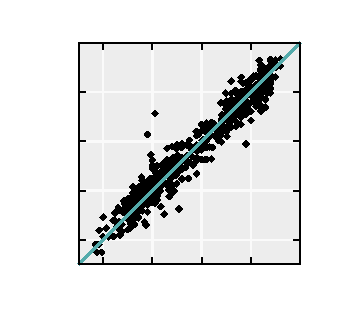
\includegraphics{gp/ms-sa-ph-corr}}%
    \gplfronttext
  \end{picture}%
\endgroup

				}
				\caption{\parbox[t]{0.43\textwidth}{
					$\widehat{\m{pH}} \sim \m{pH}$ \smallskip \\
					$(R^2)^{(\m{pH})} = 0.940$
					}}
				\label{sfig:gof-ph}
			\end{subfigure}
			\caption{Correlation diagrams plotting $\hat{y}$ on $y$ and the BLUE line representing the $\id$}
			\label{fig:gof}
		\end{figure*}
	
		Figures \ref{sfig:calib-soc}, \ref{sfig:calib-n} and \ref{sfig:calib-ph} show the selected wavelengths highlighted in grey.
		One notes that the density of selected lightwaves varies strongly along the wavelength for all three response variables, where $p^{(\m{SOC})}$ uses the most and $\m{pH}$ the lowest amount of predictors.
		
		For $p^{(\m{SOC})}$ and $p^{(\m{N})}$, we find that similar regions seem relevant for prediction, albeit the predictors for $p^{(\m{N})}$ appear to beslightly more evenly distributed along the whole bandwidth \textbf{[Is that the correct term?]}.
		In the selected model for $p^{(\m{SOC})}$, predictors are highly concentrated in the regions from 1550 - 1650 $\unit{nm}$, 1790 - 1810 $\unit{nm}$, 1980 - 1990 $\unit{nm}$, around 2500 $\unit{nm}$ and between 2600 and 2672 $\unit{nm}$.
		
		The distribution of predictors for the $\m{pH}$ appears to be highly distinct from the other two models.
		In particular, the lower-middle wavelengths seem to have more predictive power than for $p^{(\m{SOC})}$ and $p^{(\m{N})}$.
		
		Appendix \ref{sec:parameters} hosts the tables with the estimated parameters for the predictors for each model.
		It is noteworthy to inspect the values of the intercepts for each model.
		We find that these appear relatively close to commonly known \enquote{neutral} figures -- 0 in case of $p^{\m{(SOC)}}$ and $p^{\m{(N)}}$ and not too far from 7 in case of the $\m{pH}$. %albeit a distance of roughly on  1 point is still quite I assume
		
	% subsection calibration

	\subsection{Goodness of Fit}
	\label{ssec:suitability}
	
		Figure \ref{fig:gof} displays the correlation diagrams introduced in \ref{ssec:model-validation} for each response variable together with the values for the $R^2$.
		Both indicate that our estimation and model selection to predict $\m{pH}$ are working best.
		Assuming that pure error exists due to measurement, an $R^2 = 0.940$ shows a good accordance between predictions by the model and the actual observed values.
		The clear pattern in diagram \ref{sfig:gof-ph} corroborates these findings further.
		
		We have already seen on several occasions that $\m{pH}$ has to be treated slighted different from the other two response variables.
		This pattern repeats itself here as well.
		$p^{\m{(SOC)}}$ and $p^{\m{(N)}}$ display not only somewhat lower values for $R^2$, but their correlation diagrams show a common divergence from the identity.
		Our predictions seem to underestimate the observed values for the upper third of the observed interval.
		This could be due to a lack of data, which are considerably scarcer in that region than in the regions where the fits appear good.
		Only less than 5 \% of the whole measurements lie in the upper tiers of both response variables.
		
		Another reason might be that the linear assumption is misplaced, by judging from the visual aspects of the scatter plot alone.
		As we have strong reason to maintain the linear hypothesis (cf. \ref{ssec:nirs}) and taking into account that for most values the correlation seems even better than in the case of $\m{pH}$, we maintain that it is safe to assume higher measurement errors in as $p^{\m{(SOC)}}$ and $p^{\m{(N)}}$ increase, which in turn contributes to higher levels of pure error and thus to lower values of $R^2$.
		In sum, there is not sufficient evidence to reject the selected and estimated models at this point.
		
	% subsection suitability

% section model-selection